%
\documentclass[conference]{IEEEtran}
\usepackage{times}

% numbers option provides compact numerical references in the text. 
\usepackage[numbers]{natbib}
\usepackage{multicol}
\usepackage[bookmarks=true]{hyperref}
\usepackage{color}
\usepackage{graphicx}
\usepackage{textcomp}
\usepackage{amsthm}
\usepackage{amsfonts}
\usepackage{subcaption}
\usepackage{algorithm}
\usepackage{algpseudocode}

\theoremstyle{definition}
\newtheorem{definition}{Definition}[section]
\usepackage{amsmath}

\renewcommand{\algorithmicrequire}{\textbf{Input:}}
\renewcommand{\algorithmicensure}{\textbf{Output:}}

%% Tarik's Shortcuts
% For marking TODOs in an obvious way
\newcommand{\TODO}[1]{ {\bf \textcolor{red}{TODO:} #1 }}
\newcommand{\changedByJim}[1]{\textcolor{blue}{#1}}
\usepackage{amsbsy}

\begin{document}

% paper title
\title{Computer-aided design of complex configurations and behaviors for modular robots}

% You will get a Paper-ID when submitting a pdf file to the conference system
\author{Author Names Omitted for Anonymous Review. Paper-ID [add your ID here]}

\maketitle

\begin{abstract}
In this paper, we present a software framework for the compositional design of
modular robot configurations and behaviors. Designs are constructed
hierarchically by composing elements from a library, allowing users to easily
create complex designs.  Likewise, complex behaviors are constructed by
composing controllers from a library in a nested series/parallel structure. The
system is integrated with a full dynamic simulator, and provides tools to
identify common problems with behaviors, specifically self-collision and loss
of quasi-static stability.

\end{abstract}

\section{Introduction}
Modular reconfigurable robot systems have been studied extensively for several
decades \TODO{citations}.  These systems distinguish themselves in their
ability to transform into different shapes to address a wide variety of tasks.

This additional flexibility places an additional burden on the user, because
solving problems with modular robots involves not only designing  software,
but also the best physical form for the task at hand. We argue that if this
complexity is not appropriately managed, it can make the system
impractical. If the user is free to create any new design he/she pleases to
solve a new task, but must program the design from scratch every time, creating
new designs will be a huge amount of effort, and the advantage of flexible modular
hardware will be defeated.

Software modularity is a well-established practice for developing large
maintainable systems and avoiding duplication of effort \TODO{cite}. In robotics, software
behaviors are inextricably linked to the hardware they control, resulting in
additional challenges to modularity. Significant progress has been made in
sharing robotics software between researchers
and hardware platforms, most notably
ROS which provides IPC and standard libraries for common robot tasks. 

The challenges of software design are different in modular robotics than
in typical robotics, because the hardware itself is modular. Porting software
from one robot platform to a completely different robot platform takes a
considerable amount of time, and needs to be facilitated by a large framework
such as ROS, in which fundamental software libraries are almost totally decoupled from
specific hardware. In modular robotics, the emphasis needs to be on speed of
design, because the major advantage of a modular robot system is that new
designs can be made for each task. We need to  very quickly develop simple kinematic
behaviors (\textit{i.e.} take a step with a leg) with new morphologies that share some of the
structure of old morphologies.

Our solution to this problem is to let the modularity of our hardware determine the
modularity of our software. We create new modular robot designs by combining existing sub-designs,
for example combining four legs with a body to create a walking robot.
We provide a GUI tool that allows users to do this easily. Designs have
associated libraries of software behaviors, so that when new designs are created
by composing existing sub-designs, new behaviors for that design can be quickly
and easily created by composing the behaviors associate with its component
sub-designs. We introduce new scripting language with a series-parallel
execution structure that allows old behaviors to be easily and clearly combined
into new behaviors.

Since combining old things in new ways can lead to unexpected problems, we also
need to verify that our new designs and behaviors perform the way we expect them
to. This is done in a dynamic simulation in Gazebo, and through
verification tools that detect common problems.


\section{Contribution and Paper Structure}

The primary contribution of this paper is a software framework that allows modular
robot configurations and behaviors to be built hierarchically, and a simulation
environment that helps the user verify intended behavior.  Together, these tools
help manage the complexity of a modular robot system, significantly reducing the
time and effort required to accomplish tasks with modular robots.

The software we developed is open-source and freely available at\TODO{Link}.  Our
code is built for SMORES,  a modular robot developed at the University of
Pennsylvania (see sec \ref{fig:SmoresRobot}), but could easily be adapted for use with
other modular robot systems.

The remainder of this paper provides a comprehensive description of the
structure and algorithmic components of our software system.  In Section \ref{sec:related-work},
we discuss relevant background material.
In Section \ref{sec:preliminaries} we introduce terminology and  concepts used elsewhere in the
paper. 
In Section \ref{sec:approach}, we describe the algorithmic basis
for the three major components of our framework - design composition, behavior
composition, and behavior verification.  In Section
\ref{sec:example}, we discuss the open-source software
tools used to implement our system, and provide examples demonstrating a user's
workflow when using this system.  We demonstrate that our framework saves the
user time and effort, and allows him or her to easily develop complex and
capable designs.


\section{Related Work}
\label{sec:related-work}
In some respect, our work parallels the efforts of Mehta \cite{mehta2014design}
and Bezzo \cite{bezzo2014demo}, who aim to create and program printable robots from
design specification by a novice user.  Users create new designs by composing
existing elements from a design library, and appropriate circuitry and
control software are automatically generated as physical designs are assembled. The framework we present is
intended specifically for modular robots, and consequently the workflow and design considerations are fundamentally different
from that presented by Mehta and Bezzo.  In
traditional robot design (or printable robot design), hardware and software are somewhat
decoupled - hardware is
designed and built once, and then programmed many times.  In the case of a MRS, the system can be reconfigured to meet new tasks,
so hardware configuration and behavior programming go hand in hand.  We intend
our system to be fast enough that the user could conceivably develop and program
a new design for every new task - designs are built once, and programmed once.  Where Mehta et al provide many facilities to generate and verify
low-level behaviors (i.e. motor drivers appropriate for motors, we do so for
high-level behaviors.

A significant amount of work has been done in developing behaviors and software
for modular robots. Much of this work focused on automatically
generating designs and behaviors using artificial intelligence systems. Genetic
algorithms have been applied for the automated generation of designs
and behaviors \cite{hornby2003generative}. Other work has
focused on emergent behavior from distributed algorithms \TODO{cite papers}.

While significant progress has been made in the automated generation of modular robot behaviors,
automated systems are not yet capable of making modular robots truly useful in practice
\cite{yim2007modular}.  The need for new programming techniques to manage the complexity
of modular robot systems has been acknowledged in the literature \cite{yim2000modular}.
Historically, gait tables have been a commonly used format in which open-loop kinematic
behaviors can be easily encoded \cite{yim1994locomotion}. Phased automata have also
been presented as a way to easily create scalable gaits for large numbers of modular
robots \cite{zhang2003phase}. In this paper, we present a novel scripting language
to quickly create complex behaviors for modular robots.

Our framework assists users in verifying design validity by identifying self-collision
and loss of gravitational stability. Identification of these conditions is common
in modular robot reconfiguration planning \cite{casal2001reconfiguration} and motion
planning \cite{yoshida2002self}.

\section{Preliminaries}
\label{sec:preliminaries}
\subsection{SMORES robot}
We have developed our system for the SMORES modular robot, developed at the
University of Pennsylvania \cite{Davey2012}. Each SMORES modules has four DoF
(DoF) - three continuously rotating faces we call {\em turntables} and one
central hinge with a 180\textdegree\ range of motion (Figure~\ref{fig:SmoresRobot}). The
DoF marked 1, 2, and 4 have rotational axes that are parallel and coincident.
\changedByJim{Each SMORES module can drive around as a two-wheel differential
drive robot.}
SMORES modules may connect to one another via magnets on each of their four
faces, and are capable of  self-reconfiguration.

Note that while we demonstrate our software with SMORES, it is not limited to
the SMORES robot - it could be applied to any modular robot which may be
simulated using Gazebo.


\begin{figure}[tb]
    \begin{center}
        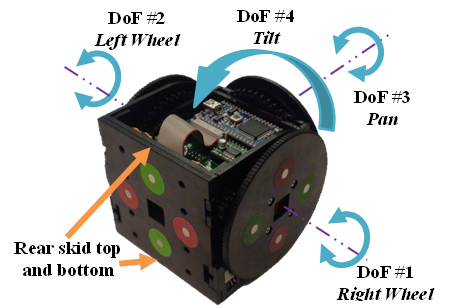
\includegraphics[width=\columnwidth]{images/smores_robot.png}
    \end{center}
    \caption{SMORES robot}
    \label{fig:SmoresRobot}
\end{figure}

\subsection{Concepts and terms}
A \textit{configuration} is a contiguous set of connected modules which we treat as a
single robot.  Configurations are defined by their connective structure, and
are represented by graphs with nodes representing modules and edges
representing connections between modules.  Edges are labeled to indicate which
faces are connected as well as any angular offset, so that all information
about the connective topology of the modules is captured.  Individual modules
are considered interchangeable (as long as they are of the same kind), so any
two identically connected sets of modules are considered instances of the same
configuration.

A \textit{behavior} is a programmed sequence of movements for a specific configuration
intended to produce a desired effect.  A gait for walking is one example.  In
this paper, we consider open-loop kinematic behaviors represented as
series-parallel action graphs, described in detail in section
\ref{sec:behavior-representation}.

A \textit{controller} is a position and velocity servo for one DoF of a modular
robot.  A controller takes as input a desired position or angular velocity, and
drives the error between the desired and actual state of the DoF it controls to
zero over time.

When writing a behavior, it is possible to command one controller to
simultaneously hold more than one desired position; this is known as a
\textit{controller conflict}.  Behaviors with controller conflicts are
impossible to execute.

During execution of a behavior, a \textit{self-collision} can occur when two
different parts of configuration are commanded to occupy the same location in
space.  Self-collisions can damage the robot, and are usually unwanted.

While executing many behaviors, it is desirable to maintain \textit{gravitational
stability} (also called quasi-static stability).  Informally speaking, a
robot is gravitationally stable when it is balanced, and gravity does not
create any net moment on it.  Mathematically, the robot is gravitationally stable
if the Z-projection of its center of
mass lies within the convex hull of its load-supporting contact points in the
ground plane.  

\section{Approach and Algorithm}
\label{sec:approach}
The three major components of our framework are configuration composition, behavior
composition, and verification of configurations and behaviors.  We begin with some definitions, and then
address each of these three components.
\begin{definition}[Module] 
We define a single module  as $\mathcal{M}=(P_{/\mathcal{R}}, O_{/\mathcal{R}}, V, N)$, where
\begin{itemize}
\item $P_{/\mathcal{R}}=(p_x,p_y,p_z)$ is the position of the module in the global reference frame $\mathcal{R}$. We consider the position the center of the module as the position of the module.
\item $O_{/\mathcal{R}}=(o_w, o_x, o_y, o_z)$ is the orientation of the module represented by quaternion in the global reference frame $\mathcal{R}$.
\item $V=\{v_1, v_2, ..., v_m\}$ is the set of joint values. Each joint value corresponds to each degree of freedom of the module.
\item $N=\{n_1, n_2, ..., n_k\}$ is the set of nodes where the module can connect to other modules.
\end{itemize}
For a single SMORES module, there are four degree of freedom as shown in Figure~\ref{fig:SmoresRobot}, and there are four nodes to connect to other modules, i.e. $N=\{$front, left, right, back$\}$ as shown in Figure~\ref{fig:smores}.

\begin{figure}
\begin{center}
        \begin{subfigure}[b]{0.4\columnwidth}
                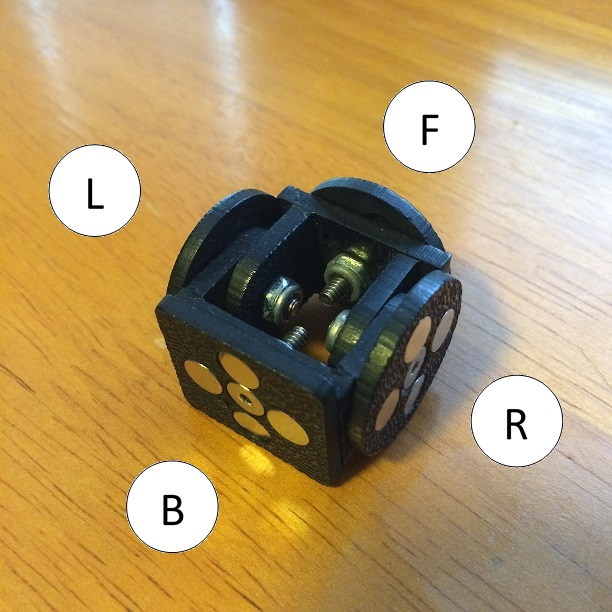
\includegraphics[width=\textwidth]{images/smores.JPG}
                \caption{A SMORES module}
                \label{fig:smores_photo}
           \end{subfigure}
           ~
        \begin{subfigure}[b]{0.4\columnwidth}
                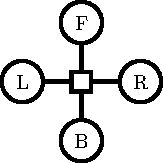
\includegraphics[width=\textwidth]{images/tikz/smores.pdf}
                \caption{The graphical representation}
                \label{fig:smores_graph}
        \end{subfigure}
\end{center}
\caption{A photo of a SMORES module and its graphical representation}
\label{fig:smores}
\end{figure}
\end{definition}

\begin{definition}[Configuration] \label{def:configuration}
We define a configuration as $\mathcal{C}=(M, \mathcal{M}_b, E, \delta)$, where
\begin{itemize}
\item $M$ is a set of modules, $M=\{\mathcal{M}_1, \mathcal{M}_2, ..., \mathcal{M}_q\}$.
\item $\mathcal{M}_b$ is single module that will be treated as a base module.
\item $E$ is a set of connections between modules. $(\mathcal{M}_i, n_i,
\mathcal{M}_j, n_j)\in E$, where $\mathcal{M}_{i,j} \in M, \mathcal{M}_i \neq
\mathcal{M}_j$, and $n_{i,j}\in N$.
\item $\delta: E \rightarrow \mathbb{R}$ is a labeling function over a
connection. Given a connection, $\delta$ returns the angle offset in degree
between the two connected nodes.
\end{itemize}
Figure~\ref{fig:smores_conf_graph} shows a photo of a configuration and its
graphical representation. Blue zigzag lines represent connections between
modules, and the label of each connection shows the angle offset of that
connection.
\end{definition}

\begin{figure}
\begin{center}
        \begin{subfigure}[b]{0.4\columnwidth}
                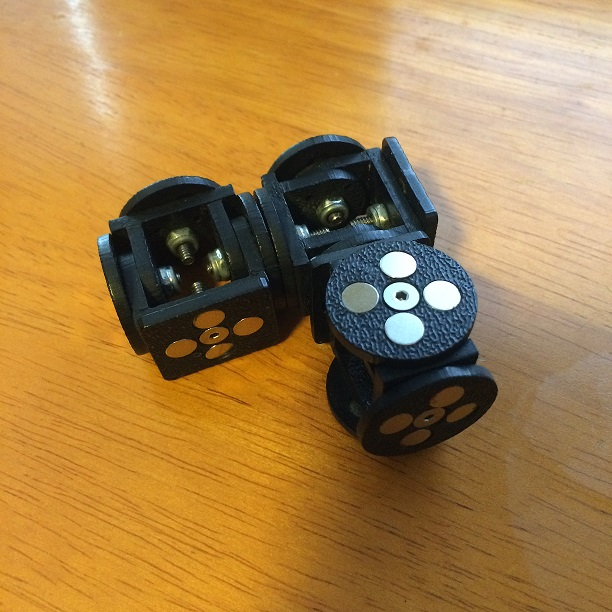
\includegraphics[width=\textwidth]{images/smores_conf.JPG}
                \caption{A configuration}
                \label{fig:smores_conf_photo}
           \end{subfigure}
           ~
        \begin{subfigure}[b]{0.4\columnwidth}
                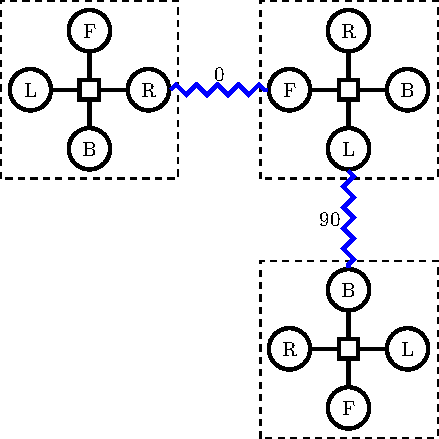
\includegraphics[width=\textwidth]{images/tikz/smores_conf.pdf}
                \caption{The graphical representation}
                \label{fig:smores_conf_graph}
        \end{subfigure}
\end{center}
\caption{A photo of a configuration with SMORES modules and its graphical representation}
\label{fig:smores_conf}
\end{figure}


\subsection{Configuration Composition} \label{sec:conf_composition}
In order to demonstrate our algorithm on configuration composition, we need to first extend the definition on configuration to allow make a configuration by composing multiple configurations.

\begin{definition}[Extended Configuration] 
We extend the definition of a configuration as $\mathcal{C}_\alpha=(C_\alpha, \gamma, M, \mathcal{M}_b, E, \delta)$, where
\begin{itemize}
\item $C_\alpha$ is a set of configurations, $C_\alpha=\{\mathcal{C}_{\alpha1}, \mathcal{C}_{\alpha2}, ..., \mathcal{C}_{\alpha q}\}$.
\item $\gamma: C_\alpha \rightarrow M$ is a function that, when given a configuration, returns all modules of that configuration.
\item $M$ is the set of modules. If this configuration contains no other configurations, i.e. $C_\alpha = \emptyset$, $M$ is just the set of all modules of this configuration as defined in Definition~\ref{def:configuration}. If this configuration is composed by other configurations, i.e. $C_\alpha=\{\mathcal{C}_{\alpha1}, \mathcal{C}_{\alpha2}, ..., \mathcal{C}_{\alpha q}\}$, we define $M=\bigcup_{\mathcal{C}_{\alpha}\in C_{\alpha}}{\gamma(\mathcal{C}_{\alpha})}$.
\item $\mathcal{M}_b\in M$ is a single module that will be treated as a base module.
\item $E$ is a set of connections between modules. $(\mathcal{M}_i, n_i, \mathcal{M}_j, n_j)\in E$, where $\mathcal{M}_{i,j} \in M, \mathcal{M}_i \neq \mathcal{M}_j$, and $n_{i,j}\in N$.
\item $\delta: E \rightarrow \mathbb{R}$ is a labeling function over a connection. Given a connection, $\delta$ returns the angle offset in degree between the two connected nodes.
\end{itemize}
\end{definition}
The extended configuration can represent a complex structure with nested configurations with arbitrary depth. For the rest of the paper, we will omit the subscript $\alpha$, and use $\mathcal{C}$, $C$ to stand for ``one extended configuration'' and ``a set of extended configurations'' respectively.

\begin{definition}[Configuration Composition] 
Given a set of configurations $C$, a base configuration $\mathcal{C}_b\in C$, and a set of connections $E_C$ that encodes the connections between configurations in $C$, configuration composition combines all configuration in $C$ to a single configuration $\mathcal{C}^*$ that has the following guarantees: i) $\mathcal{C}^*$ includes all modules and connections from $C$ and $E_C$ (section~\ref{sec:update_connection}); ii) the positions of all modules in $\mathcal{C}^*$ are adjusted based on the connections to preserve structures of original configurations in $C$ (section~\ref{sec:update_position}); iii) $\mathcal{C}^*$ is a safe configuration as defined in section~\ref{sec:safe_conf}. 
\end{definition}

\subsubsection{Update Modules and Connections} \label{sec:update_connection}
Before presenting the procedure to update modules and configurations in $\mathcal{C}^*$, we will first discuss some assumptions about the set of connections $E_C$.

The set of connections $E_C$ between configurations in $C$ is defined as $(\mathcal{C}_i, \mathcal{M}_i, n_i, \mathcal{C}_j, \mathcal{M}_j, n_j) \in E_C$, where $\mathcal{C}_{i,j}\in C$, $\mathcal{M}_i \in \gamma(\mathcal{C}_i), \mathcal{M}_j \in \gamma(\mathcal{C}_j)$, and $n_{i,j} \in N$. In addition, we assume the connections in $E_C$ form a tree structure with the configurations in $C$. That means, if we form an undirected graph by treating configurations in $C$ as nodes and connections in $E_C$ as edges, the graph should not have any simple cycle (\TODO{cite, diagram?}).

Given a set of configurations $C$, a base configuration $\mathcal{C}_b\in C$, and a set of connections $E_C$, we define the composed configurations to be $\mathcal{C}^*=(C^*, \gamma, M, \mathcal{M}_b, E, \delta)$, where
\begin{itemize}
\item $C^*=C$
\item $M=\bigcup_{\mathcal{C}\in C^*}{\gamma(\mathcal{C})}$.
\item $\mathcal{M}_b\in M$ is the base module of the base configuration $\mathcal{C}_b$.
\item $E= (\bigcup_{(\mathcal{C}_i, \mathcal{M}_i, n_i, \mathcal{C}_j, \mathcal{M}_j, n_j)\in E_C}{\{(\mathcal{M}_i, n_i, \mathcal{M}_j, n_j)}\})$ $\cup$ $(\bigcup_{\mathcal{C} \in C^*}{E}$ of $\mathcal{C})$
\end{itemize}
The definitions of $\gamma$ and $\delta$ are the same as the ones in Definition~\ref{def:configuration}.

\subsubsection{Update Positions of all Modules} \label{sec:update_position}
As multiple configurations are combined, positions and orientations of some modules in them need to be changed to preserve the relative positioning between modules as in the original configurations.

\begin{algorithm}
\caption{Update Module Position}\label{alg:update_position}
\begin{algorithmic}[1]
\Require
\Statex A parent module $\mathcal{M}_p$
\Statex A child module $\mathcal{M}_c$
\Statex A connection $(\mathcal{M}_p, n_p, \mathcal{M}_c, n_c)$ and labeling function $\delta$
\Ensure
\Statex The child module $\mathcal{M}_c$ with position and orientation updated
\Statex
\State c\_wrt\_p $\gets$ get\_transform($V_p$, $V_c$, $n_p$, $n_c$)
\State p\_wrt\_world $\gets$ get\_matrix($P_p$, $O_p$)
\State c\_wrt\_world $\gets$ p\_wrt\_world $\cdot$ c\_wrt\_p
\State $P_c \gets$ get\_position(c\_wrt\_world)
\State $O_c \gets$ get\_orientation(c\_wrt\_world)
\State Update $\mathcal{M}_c$ with $P_c$ and $O_c$
\end{algorithmic}
\end{algorithm}


\paragraph{Configuration composition}
Define the composition of a set of configurations to a single configuration.

\TODO{Jim writes}
\paragraph{Input}
A set of configurations. A topology graph representing the connectivity among those configurations. A base module (for position transformation).
\paragraph{Output}
A composed configuration if it is safe.
\paragraph{Procedure}
\begin{itemize}
\item Start from the configurations that connects to the configuration with base module, transform their positions based on the position of the base configuration and topology graph.
\item Check if there is any collisions among the modules and report such collision.
\item \textbf{Check if the final configuration is stable. If not, find the plane that will make the configuration stable and transform the configuration.}
\item Show the expected behavior in simulator.
\end{itemize}

\paragraph{Controller composition}
Define the composition of a set of controllers to a single controller. Define the difference between a parallel composition and a series composition. Define the control composition graph.

\subsection{Behavior Composition: Series-Parallel Action Graphs}
\label{sec:behavior-representation}
We present a novel motion description language for modular robots.  The
language aims to balance simplicity and expressiveness, and is compositional in
nature, designed to manage the complexity of developing complicated behaviors
for large clusters of modular robots through abstraction and modularity. The language
is in some ways similar to typical extended motion description languages (see \cite{hristu2003motion}),
but was specifically designed to facilitate  composition.
 
The fundamental atoms of the language are called actions.  An \textit{action} is a tuple \(
(J, X, \xi, T)\), where \(J\) identifies a single DoF of a configuration, \(X\) is a
controller setpoint for that degree of freedom, \(\xi\) specifies an interrupt
condition, and T specifies a timeout. When an action executes, the controller
setpoint (position or velocity) for the specified DoF is changed to the specified
value. The controller maintains this setpoint until receiving a new one from another
action. 

The interrupt condition is a boolean function of the (sensed) state of the DoF \(J\).
When either the interrupt condition is met or time runs out (whichever comes
first), the action is considered complete, and the next action  begins. The
interrupt condition can be set to \(false\) (so that only the timeout has effect),
and \(T\) can be set to infinity (so that only the interrupt has effect).

Actions are composed to form behaviors. We define a \textit{behavior} as a directed acyclic graph where nodes are
actions and edges are transitions between actions.  A behavior \(B\) always has
two special nodes \(S\) and \(T\), which are the \textit{Start} and
\textit{Termination} nodes, respectively.  The smallest behavior consists of
\(S\), \(T\), and a single action.  Behavior execution follows three simple
rules:

\begin{enumerate}
\item Execution begins at \(S\).  \(S\) completes immediately.
\item Each action begins execution upon completion of \textit{all} its parent actions.
\item All sequences of execution end at \(T\).
\end{enumerate}

Because execution begins at \(S\) and ends at \(T\), there must be a (directed)
path from every \(S\) to every node in \(B\), and also from every node in \(B\)
to \(T\). Since \(B\) is acyclic, it is therefore a \textit{directed series-parallel graph} (SPG).
SPG's can always be formed recursively by parallel and series composition
operations \cite{valdes1979recognition}. The parallel composition \(P\) of two behaviors \(B_1\),
\(B_2\), \(P = Pc(B_1, B_2)\) is the disjoint union of their nodes (actions),
merging \(S_1\) with \(S_2\) and \(T_1\) with \(T_2\). The series composition
of \(B_1\), \(B_2\), \(S = Sc(B_1, B_2)\) is created from their disjoint union
by merging \(T_1\) and \(S_2\), so that \(B_1\) and \(B_2\) execute
sequentially\footnote{Since the merged node is not an action, we can freely
omit it and instead draw edges from each of its parent nodes to each of its
child nodes.}.  Note that if \(B_1\) was itself created through parallel
composition, \(B_2\) will not begin until all chains of execution of \(B_1\)
are completed. Figure \ref{fig:graph-composition} provides a visual companion.

\begin{figure}
\begin{center}
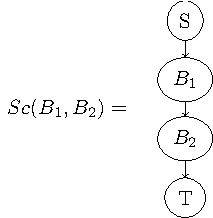
\includegraphics[height=0.8in]{images/tikz/series.pdf}
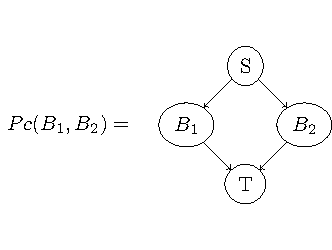
\includegraphics[height=0.8in]{images/tikz/parallel.pdf} \vspace{0.in}
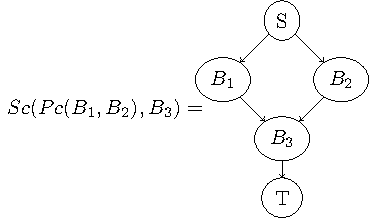
\includegraphics[height=0.8in]{images/tikz/parallel-and-series.pdf}
\end{center}
\caption{Series and parallel composition of behaviors }
\label{fig:graph-composition}
\end{figure}

\subsubsection*{Example}
A single SMORES module can use its left and right wheels to drive like a car. To
drive forward, we might define a DRIVE behavior composing actions for  the left and right wheels
in parallel:\begin{align*}
\mathrm{DRIVE} =~~~~~~~~~~~~~~~~~~~~~~~~~~~~~~~~~~~~~~~~~~~~~~~~~~~ \\
Pc \left( \begin{array}{cccc}
(~L, & \dot\theta_{set}=6, & \xi:false, & T:5), \\
(~R, & \dot\theta_{set}=6, & \xi:false, & T:5) \\
\end{array} \right)\\
\end{align*}
The wheels are set to turn at 6 radians per second, and the action will complete
in 5 seconds.  We might also define a TURN behavior, commanding the wheels to rotate \(\pi\) radians
in opposite directions:
\begin{align*}
\mathrm{TURN} =~~~~~~~~~~~~~~~~~~~~~~~~~~~~~~~~~~~~~~~~~~~~~~~~~~~~~~~~~~~~ \\
Pc \left( \begin{array}{cccc}
(~L, & \theta_{set}=\theta_0+\pi, & \xi:\theta==\theta_0+\pi, & T:\infty), \\
(~R, & \theta_{set}=\theta_0-\pi, & \xi:\theta==\theta_0-\pi, & T:\infty) \\
\end{array} \right)\\
\end{align*}

Here, \(\theta_0\) denotes the currently-sensed value of theta at the beginning of
the TURN behavior.
The action completes when both wheels actually reach their commanded angles of \(\theta_0\pm\pi\). To drive in a square, we compose DRIVE and TURN behaviors in series:

\begin{align*}
\mathrm{SQUARE} = Sc (~\mathrm{DRIVE},~\mathrm{TURN},~\mathrm{DRIVE},~\mathrm{TURN},\\
~\mathrm{DRIVE},~\mathrm{TURN},~\mathrm{DRIVE},~\mathrm{TURN} )
\end{align*}

% Consider the
% car design shown in Figure X. This design is composed of four wheel modules
% and a central steering element, which rotates to bend the front wheels to the
% left or right relative the back, causing the car to turn. The wheel elements
% expose a function which turns the two side turntables in sync in order to drive
% forward (DRV). The steering element exposes a steering function (STR). We
% show these behavior  definitions below:
% \begin{align*}
% %
% \mathrm{DRV}(v,t) =~~~~~~~~~~~~~~~~~~~~~~~~~~~~~~~~~~~~~~~~~~~~~~~~~~~ \\
% Pc \left( \begin{array}{cccc}
% (~lWheel, & \dot\theta=v, & \xi:0, & T:t~), \\
% (~rWheel, & \dot\theta=v, & \xi:0, & T:t~) \\
% \end{array} \right)\\
% %
% \mathrm{ST R}(x) = ~~~~~~~~~~~~~~~~~~~~~~~~~~~~~~~~~~~~~~~~~~~~~~~~~~~~ \\ 
% Pc \left( \begin{array}{cccc}
% (~tTable1 & \theta=x, & \xi:[\theta=x], & T=\infty~), \\
% (~tTable2 & \theta=-x, & \xi: [\theta=-x], & T=\infty~) \\
% \end{array} \right)
% %
% \end{align*}
% 
% The DRV behavior sets an angular velocity \(v\) for the left and right 
% 
% After composing these sub-configurations into the car, we build higher-level
% behaviors by composing the behaviors of the sub-configurations. We define functions
% to go-straight (GST) and turn (TRN):
% \begin{align*}
% \mathrm{GST}(v,t) &= Pc (~\mathrm{STR}(0),~ \mathrm{DRV}(v,t)~)\\
% \mathrm{TRN}(v,t,x) &= Pc (~\mathrm{STR}(x),~\mathrm{DRV}(v,t)~)
% \end{align*}
% 
% We can now easily define trajectories by sequencing go-straight and turn
% commands in series. Figure \ref{fig:zigzag} shows the path generated by the
% zig-zag behavior defined below:
% 
% \begin{align*}
% ZGZ = ~~~~~~~~~~~~~~~~~~~~~~~~~~~~~~~~~~~~~~~~~~~~~~~~~~~~~~~~~\\
% Sc(~\mathrm{GST}(10,5),~\mathrm{TRN}(10,5,30),~\mathrm{GST}(10,5),\\
% ~\mathrm{TRN}(10,10,-30),~\mathrm{GST}(10,20), \\
% \mathrm{TRN}(10,10,30), \mathrm{GST}(10,5), \mathrm{TRN}(10,10, -30 )~)
% \end{align*}
% 
% \begin{figure}
% \begin{center}
% 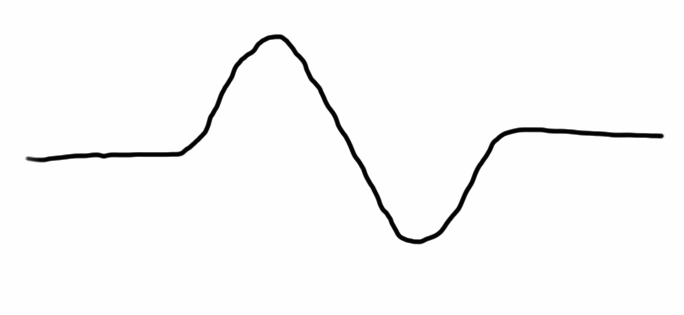
\includegraphics[width=0.7\columnwidth]{images/zigzag.png}
% \end{center}
% \caption{Zig-zag trajectory \TODO{This is hand-drawn, sorry about that... I will
% make a more professional-looking replacement}}
% \label{fig:zigzag}
% \end{figure}
 
% \subsection{Controller Composition}
% \TODO{Tarik and Jim write}
% \paragraph{Input}
% A configurations. A set of controllers. A control composition graph.
% \paragraph{Output}
% A composed controller if it is safe.
% \paragraph{Procedure}
% \begin{itemize}
% \item Compose the set of controllers based on the given control composition graph. Explain how the parallel composition and series composition are handled.
% \item\textbf{Check there is no controller conflict in the composition.}
% \item Execute the composed controller in user defined incremental time interval. At each time step, update each module position and check collision.
% \item \textbf{At each time step, check if the configuration will not have any unexpected behavior.}
% \end{itemize}

\subsection{ Verification of Configurations and Designs}
\TODO{Jim writes}

\subsection{Complexity}
Discuss the complexity of the algorithm with respect to the number of modules and size of gait tables.

\section{Implementation }
\label{sec:example}
\TODO{Tarik and Jim write}\\
With simulation in Gazebo:
\begin{itemize}
\item Show a configuration composed from a set of basic configurations.
\item Show a composed controller that results in a collision in the configuration.
\item Show an updated controller that resolves the collision
\item Show a composed controller that results in an unexpected behavior.
\item Show an updated controller that eliminates the unexpected behavior.
\end{itemize}

\section{Examples}
Here we present some examples to illustrate important features of our framework.
\subsection{Toward a Standard Library}
Our eventual intention is to develop a large library of configurations and associated
behaviors which are available to all users of our framework, analogous to the standard
libraries of major programming languages.  The compositional nature of our framework
will allow users to rely heavily on the library when approaching new tasks, allowing
them to create sophisticated robots very quickly.

As a first step toward a standard library, we present a small library of configurations
and associated behaviors in Tables \ref{Order-1-configurations} and \ref{Order-2-configurations}.
Configurations in the library are organized by \textit{order}, defined recursively
as follows: a single module is an order-zero configuration, and the order of all
other configurations is one greater than the largest order of the sub-configurations
from which it is composed. Associated with each configuration is a set of behaviors. \TODO{Behaviors are grouped
by functionality?}.

For the library to be most effective, the set of configurations and behaviors available
 at each level (and especially at the lowest levels) should provide a rich set of
 functionalities without presenting the user with an overwhelming number of options. 
 Considering the small library in Tables \ref{Order-1-configurations} and \ref{Order-2-configurations},
 it is interested to note that a large  and diverse set of second- and third-order configurations can
be constructed from only three first-order configurations. Developing metrics to
evaluate the quality of such a library is an interesting opportunity for future work. 

\begin{table*}
    \begin{center}
        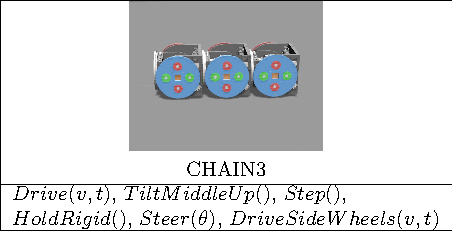
\includegraphics[width=\textwidth]{images/library/tier1.pdf}
        \caption{Tier-1 configurations (basic configurations)}
        \label{Order-1-configurations}
    \end{center}
\end{table*}
\begin{table*}
    \begin{center}
        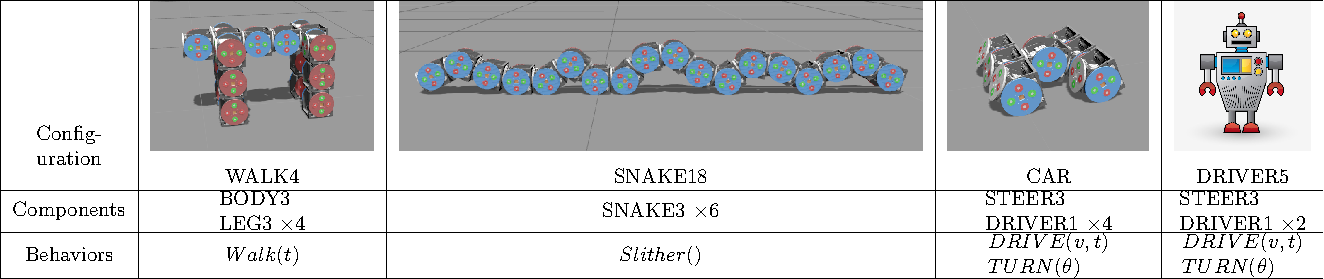
\includegraphics[width=\textwidth]{images/library/tier2.pdf}
        \caption{Tier-2 configurations (composed of basic configurations)}
        \label{Order-2-configurations}
    \end{center}
\end{table*}

\subsection{The User Perspective}
We present the start-to-end user perspective in designing a complicated configuration,
called Walkbot. \TODO{Jim, can you write this section?}

\subsection{Easy scale-up through composition}
Our framework allows users to quickly create and program large configurations. The
first order CHAIN3 configuration (Figure \ref{fig:chain3}) can use a \(sineGait\)
behavior to locomote like a snake. Defining \(sineGait\)  as the series composition
of two half-waves will allow us to re-use the gait with larger snakes:
\begin{displaymath}
sineGait = Sc(~halfSine1,~halfSine2~)
\end{displaymath}
Arbitrarily long snake configurations can be created
by composing CHAIN3's end-to-end; Figure \ref{fig:snake18} shows one with 18 modules.
A gait for an arbitrarily long snake is created by composing sine wave
gaits for each component in parallel, but with alternating phase:
\begin{align*}
nSnakeSineGait = ~~~~~~~~~~~~~~~~~~~~~~~~~~~~~~~~~~~~~~~~~~\\
Pc \left(~Sc\begin{pmatrix} halfSine1 \\ halfSine2 \end{pmatrix},
~Sc\begin{pmatrix} halfSine2 \\ halfSine1 \end{pmatrix},\ldots ~\right)
\end{align*}
\subsection{Verification}
The need for verification becomes more important as design complexity increases.
 Consider the Backhoe design, composed of the 2nd-order car and PUMA arm configurations.
 It is easy for this design to become gravitationally unstable.  Our verification
 system warns the user when this happens.

\section{Results}
In the past, designing configurations and behaviors to address new tasks has required
time on the order of one day \cite{sastra2011using}. Using our framework and library,
complex designs (such as the Walkbot or 18-module snake) can be created and programmed
in under an hour. \TODO{Mark, what is the best
way to present this comparison?} 

\section{Conclusions}
We worked hard, and had fun.

\section{Future}
\begin{itemize}
\item How to represent different attribute/ability of the configurations
\end{itemize}




%% Use plainnat to work nicely with natbib. 

\bibliographystyle{plainnat}
\bibliography{references}

\end{document}



